\subsection*{\Large Общая характеристика работы}
\fontsize{14pt}{15pt}\selectfont
\underline{\textbf{Актуальность темы.}}
Сердечно-сосудистые заболевания являются одной из наиболее острых проблем современного общества. Во всех странах их количество существенно опережает остальные, поэтому трудно переоценить значимость исследований в этой области. В последние годы наблюдается резкий рост интереса к проблеме сердечно-сосудистых заболеваний, развиваются новые методики исследования, появляются все более точные измерительные приборы. Каждый год в мире проводится примерно 250 000 операций восстановлению или замене поврежденных сердечных клапанов [1] и ожидается, что в ближайшие годы это значение будет только увеличиваться [2]. При этом многие сложности, связанные с созданием искусственных клапанов или протезированием сосудов, относятся к динамике течения крови внутри. Поэтому математическое моделирование данных явлений позволяет получить более глубокое понимание происходящих процессов и найти пути усовершенствования их конструкции. 

При изучении подобных явлений методами математического моделирования зачастую удовлетворительные результаты можно получить с помощью модели вязкой несжимаемой жидкости, которая описывается системой дифференциальных уравнений Навье-Стокса, выписанных в форме естественных переменных <<скорость-давление>>. Помимо этого требуется учесть, что кровь является неоднородной по своей природе и состоит из плазмы и форменных элементов (лейкоциты, эритроциты и т.д.), а сосуды и клапаны являются гибкими и изменяют форму под воздействием различных параметров. Необходимость описывать взаимодействия гибких непроницаемых тканей с неоднородной жидкостью приводит к существенным трудностям при постановке задачи и ее численном решении, связанными с построением расчетной сетки и ее изменением в соотвтетсвии с движением лепестков клапана и деформацией сосуда. 

Существует несколько устоявшихся подходов, для того, чтобы избежать эти трудности. В данном исследовании используется метод погруженной границы, который предназначен для моделирования тонких препятствий произвольной жесткости. Это позволяет численно решать прикладные задачи оптимизации структуры искусственного клапана.


\underline{\textbf{Целью}} данной работы является разработка технологии решения нестационарной трехмерной задачи о течении неоднородной вязкой несжимаемой жидкости в крупных кровеносных сосудах с гибкими стенками и трехстворчатых клапанах с гибкими лепестками. Для достижения этой цели был создан программный комплекс, с помощью которого можно моделировать работу клапана, деформацию стенок кровеносных сосудов и получать картины течения внутри них.

\underline{\textbf{Основные положения, выносимые на~защиту:}}
\begin{enumerate}
 \item Первое положение.
 \item Второе положение.
 \item Третье положение.
% и так далее, если нужно
\end{enumerate}

\underline{\textbf{Научная новизна:}}
\begin{enumerate}
 \item Впервые ... . 
 \item Впервые ... .
 \item Впервые ... . 
\end{enumerate}

\underline{\textbf{Практическая значимость}} диссертационной работы определяется ...

\underline{\textbf{Достоверность}} изложенных в работе результатов обеспечивается ...

\underline{\textbf{Апробация работы.}}
Основные результаты работы докладывались~на:
Название симпозиума (Страна, город, год),
Название конференции (Страна, город, год),
% и так далее, если нужно

Диссертационная работа была выполнена при поддержке грантов ...

\underline{\textbf{Личный вклад.}} Автор принимал активное участие ...

\underline{\textbf{Публикации.}} Основные результаты по теме диссертации изложены в ХХ печатных изданиях, Х из которых изданы в журналах, рекомендованных ВАК, ХХ --- в тезисах докладов.

%\underline{\textbf{Объем и структура работы.}} Диссертация состоит из~введения, четырех глав, заключения и~приложения. Полный объем диссертации \textbf{ХХХ}~страниц текста с~\textbf{ХХ}~рисунками и~5~таблицами. Список литературы содержит \textbf{ХХX}~наименование.

%\newpage
\subsection*{\Large Содержание работы}
Во \underline{\textbf{введении}} обосновывается актуальность исследований, проводимых в рамках данной диссертационной работы, приводится обзор научной литературы по изучаемой проблеме, излагаются цели и задачи исследования.

\underline{\textbf{Первая глава}} посвящена описанию используемой математической модели, применяемым методам решения, разностным схемам. Рассматривается система дифференциальных уравнений Навье-Стокса, которая моделирует нестационарную задачу о течении вязкой неоднородной несжимаемой жидкости под воздействием перепада давления:

\begin{gather}
    \label{eq:navier_stokes:motion}
    \frac{\partial \vec{u}}{\partial t} + (\vec{u} \cdot \nabla) \vec{u} = - \frac{1}{\rho} \nabla p + \nabla \sigma + \vec{f}\\
    \label{eq:navier_stokes:continuity}
    \frac{\partial \rho}{\partial t} + \nabla \cdot (\rho \vec{u}) = 0 
\end{gather}

с начальными и краевыми условиями:

\begin{gather}
    \label{eq:navier_stokes:velocity_conditions}
    \vec{u}(\bar{x}, 0) = \vec{u}_0 \qquad \vec{u}|_{\Gamma_1, \Gamma_4} = \vec{u}_b \qquad u_{\Gamma_2, \Gamma3} = 0\\
    \label{eq:navier_stokes:pressure_conditions}
    p_{\Gamma_2} = p_{in} \qquad p_{\Gamma_3} = p_{out}
\end{gather}

где $\bar{x}=(x,y,z) \in \Omega$, $\vec{u}=(u,v,w)$ - вектор скорости, $\vec{u}_b$ - скорость, с которой двигаются стенки сосуда и створки клапана при деформации,
$\rho=\rho(\bar{x}, t)$ - плотность, $p=p(\bar{x}, t)$ - давление, $\sigma = \mu (\nabla \vec{u} + (\nabla \vec{u})^T)$ - вязкий тензор напряжений,
$\mu = \mu(\bar{x}, t)$ - вязкость жидкости, $\vec{f} = \vec{f}(\bar{x}, t)$ - вектор массовых сил, который в дальнейшем используется для определения формы сосуда и створок клапана. 

Область $\Omega$ изображена на рис. \ref{img:boundaries} и представляет собой сосуд с границей $\Gamma = \Gamma_1 \cup \Gamma_2 \cup \Gamma_3 \cup \Gamma_4$,
где $\Gamma_1$ - стенка кровеносного сосуда, $\Gamma_2$ и $\Gamma_3$ -  области втекания и вытекания, $\Gamma_4$ - створки клапана.

\begin{figure}[h] 
  \center
  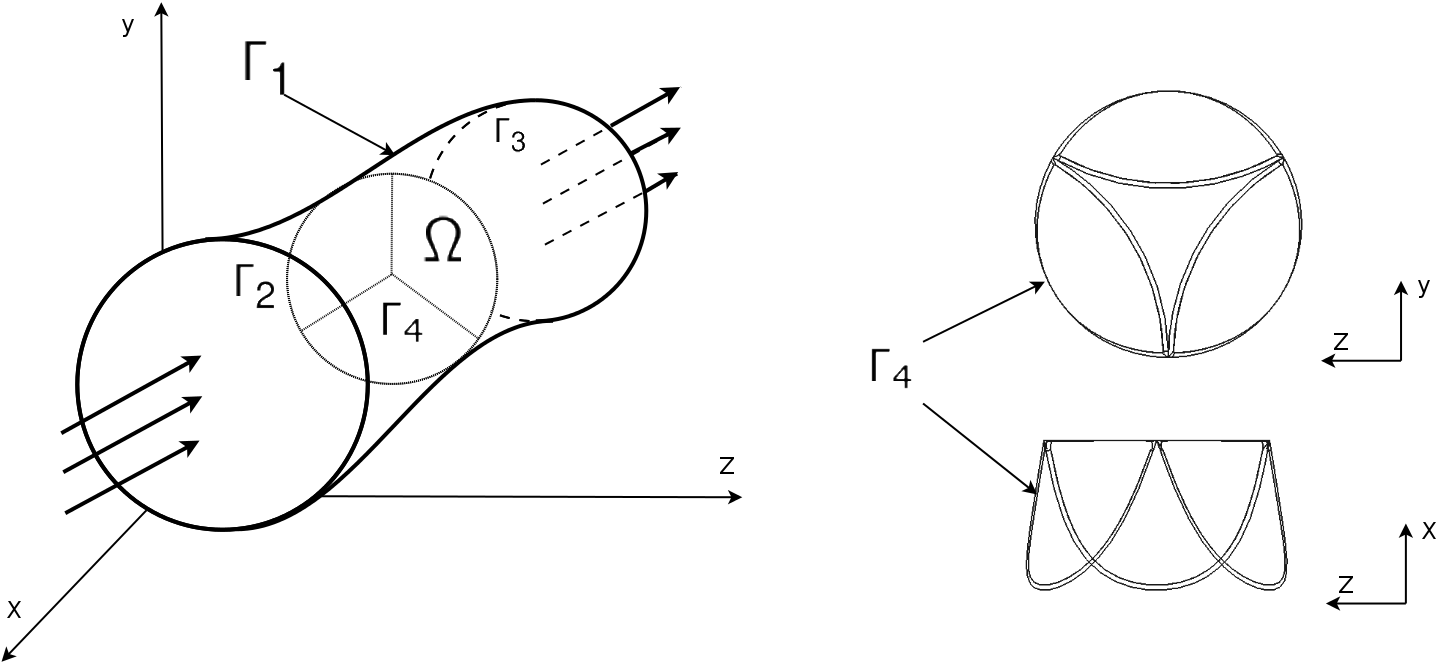
\includegraphics [scale=0.27] {area_3d.png}
  \caption{Изображение границ расчетной области} 
  \label{img:boundaries}
\end{figure}

Плотность $\rho$ и вязкость $\mu$ определяются следующими соотношениями:

\begin{gather}
    \label{eq:viscosity}
    \mu = c (\mu_2 - \mu_1) + \mu_1\\
    \label{eq:density}
    \rho = c (\rho_2 - \rho_1) + \rho_1
\end{gather}

где $\rho_1$, $\mu_1$ - плотность и вязкость жидкости (плазмы), $\rho_2$, $\mu_2$ - плотность и вязкость примеси (форменных элементов), $c$ - концентрация примеси.
Концентрация $c=c(\bar{x}, t)$, $c \in [0, 1]$ примеси определяется как решение уравнения:

\begin{gather}
    \label{eq:convection}
    \frac{\partial c}{\partial t} + \vec{u} \cdot \nabla c = 0
\end{gather}

с начальными условиями и краевыми условиями на границе втекания:

\begin{gather}
    \label{eq:convection:conditions}
    c(\bar{x}, 0) = c_0(\bar{x}), \bar{x} \in \Omega \qquad c(\bar{x}, t)|_{\Gamma_2} = c_s(\bar{x}, t)
\end{gather}

В качестве заключительного этапа описания математической модели приводятся формулы (\ref{eq:boundary_force}), (\ref{eq:interaction:velocity}, (\ref{eq:interaction:force}), используемые для моделирования взаимодействия течения жидкости и непроницаемых гибких стенок:

\begin{gather}
    \label{eq:boundary_force}
    F = \frac{\partial}{\partial s} (T \tau) + \frac{\partial^2}{\partial s^2} (E \cdot I \frac{\partial^2}{\partial s^2} X)
\end{gather}

где 

\begin{gather}
    \label{eq:interaction:velocity}
    \frac{\partial X}{\partial t}(\bar{q}, t) = \int_{\Omega} \vec{u}(\bar{x}, t) \cdot \delta (x - X(\bar{q}, t))\; dx\; dy\; dz\\
    \label{eq:interaction:force}
    \vec{f}(\bar{x}, t) = \int_{\Gamma} \vec{F}(\bar{q}, t) \cdot \delta (x - X(\bar{q}, t))\; dq\; dr\; ds
\end{gather}

где


Для поставленной задачи приводятся известные теоремы о существовании и единственности решения.

Формулы в строку без номера добавляются так:
$$
  \lambda_{T_s} = K_x\frac{d{x}}{d{T_s}}, \qquad
  \lambda_{q_s} = K_x\frac{d{x}}{d{q_s}},
$$

\underline{\textbf{Вторая глава}} посвящена исследованию 

\underline{\textbf{Третья глава}} посвящена исследованию 

В \underline{\textbf{четвертой главе}} приведено описание 

В \underline{\textbf{заключении}} приведены основные результаты работы, которые заключаются в следующем:
\begin{enumerate}
 \item Результат номер один.
 \item Результат номер два.
 \item Результат номер три.
% и так далее, если нужно
\end{enumerate}


%\newpage
\renewcommand{\refname}{\Large Публикации автора по теме диссертации}
\nocite{*}
\bibliography{biblio}
